% !TeX TS-program = xelatex

\documentclass[compress, 8pt]{beamer}

\usepackage{presentationtemplate}
\usepackage[askip=3mm, bskip=3mm]{terminal}
\usepackage[linenosfontsize=\tiny, askip=3mm, bskip=3mm]{mylisting}
\usepackage{tikz}
\usetikzlibrary{positioning}

\title{Виртуальные методы и полиморфизм}

\begin{document}

\frame[plain]{\titlepage}

\begin{frame}[fragile]

    \frametitle{Виртуальные методы}

    \hfill\break
    Механизм \textbf{виртуальных методов} (virtual members) позволяет вызывать
    методы производного класса, используя указатель или ссылку на объект
    базового класса.

    \begin{columns}

        \begin{column}{0.5\textwidth}

            \myinputlisting[minted language=cpp]
                {Presentations/13-Virtual-members/basic-example/}
                {employee.hpp}

        \end{column}

        \begin{column}{0.5\textwidth}

            \myinputlisting[minted language=cpp]
                {Presentations/13-Virtual-members/basic-example/}
                {main.cpp}

        \end{column}

    \end{columns}

\end{frame}

\begin{frame}[fragile]

    \frametitle{Полиморфизм}

    В С++ виртуальные методы являются одним из механизов поддержки
    \textbf{полиморфизма} (polymorphism): способности одного и того же
    кода работать с объектами разных типов.

    \hfill\break
    Для использования этой возможности необходимо выполнение двух условий:

    \begin{itemize}
        \item объект должен управляться через ссылку или указатель;
        \item вызываемый метод должен быть виртуальным.
    \end{itemize}

\end{frame}

\begin{frame}[fragile]

    \frametitle{Ключевое слово \texttt{virtual}}

    \hfill\break
    Для того, чтобы метод был виртуальным, достаточно ключевого слова
    \verb|virtual|\footnotemark{} в объявлении метода в базовом классе.
    Допускается использование \verb|virtual| в объявлениях методов
    классов-наследников, но оно не имеет эффекта и не рекомендуется.

    \footnotetext{\url{https://en.cppreference.com/w/cpp/language/virtual}}

    \begin{myinplacelisting}[minted language=cpp]
struct Base {
    virtual void Foo(); // virtual обязательно
};

struct Derived : Base {
    void Foo(); // эквивалентно virtual void Foo();
    virtual void Bar(); // virtual обязательно
};

struct Derived2 : Derived {
    virtual void Foo(); // эквивалентно void Foo();
    void Bar(); // эквивалентно virtual void Bar();
};
    \end{myinplacelisting}

\end{frame}

\begin{frame}[fragile]

    \frametitle{Ключевое слово \texttt{override}}

    Чтобы гарантировать, что производный класс действительно переопределяет
    существующий в базовом классе виртуальный метод, можно использовать ключевое
    слово \texttt{override}\footnotemark{}.

    \footnotetext{\url{https://en.cppreference.com/w/cpp/language/override}}

    \begin{myinplacelisting}[minted language=cpp]
struct Base {
    virtual void Foo();
    void Bar(); // ошибка: забыли ключевое слово virtual
};

struct Derived : Base {
    void Foo() override;
    void Bar() override; // ошибка компиляции
};
    \end{myinplacelisting}

\end{frame}

\begin{frame}[fragile]

    \frametitle{Ключевое слово \texttt{final}}

    \hfill\break
    С помощью ключевого слова \verb|final|\footnotemark{} можно запретить переопределять
    виртуальный метод в произвольных классах или запретить наследоваться от
    класса.

    \footnotetext{\url{https://en.cppreference.com/w/cpp/language/final}}

    \begin{myinplacelisting}[minted language=cpp]
struct Base {
    virtual void Foo();
};

struct Derived : Base {
    void Foo() final;
};

struct Derived2 : Derived {
    void Foo() override; // ошибка компиляции
};

struct Derived3 final : Base {};
struct Derived4 : Derived3 {}; // ошибка компиляции
    \end{myinplacelisting}

\end{frame}

\begin{frame}[fragile]

    \frametitle{Виртуальная таблица}

    \hfill\break
    Для каждого полиморфного типа в памяти программы создается
    \textbf{виртуальная таблица} (virtual table), в которой лежат адреса
    виртуальных методов.
    Объект полиморфного типа всегда содержит указатель на виртуальную таблицу.

    \begin{columns}

        \begin{column}{0.5\textwidth}

            \begin{myinplacelisting}[minted language=cpp]
struct Base {
    virtual void Foo() {};
    virtual void Bar() {};
};

struct Derived : Base {
    void Foo() override {};
};

void call(Base& obj) {
    obj.Foo(); obj.Bar();
}

int main() {
    Base b1 {}; call(b1);
    Base b2 {}; call(b2);
    Derived d {}; call(d);
}
            \end{myinplacelisting}

        \end{column}

        \begin{column}{0.5\textwidth}

            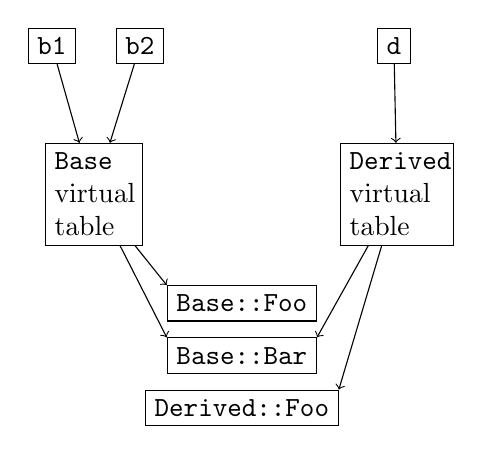
\begin{tikzpicture}
                \tikzstyle{every node}=[draw]
                \node (b1)                                                              { \verb|b1| };
                \node (b2)      [right=0.5cm of b1]                                     { \verb|b2| };
                \node (d)       [right=2.7cm of b2]                                     { \verb|d| };
                \node (bvtable) [below right=1.0cm and -0.4cm of b1, text width=1cm]    { \verb|Base| \\ virtual \\ table };
                \node (dvtable) [right=2.5cm of bvtable, text width=1.2cm]              { \verb|Derived| \\ virtual \\ table };
                \node (bfoo)    [below right=0.5cm and 0.3cm of bvtable]                { \verb|Base::Foo| };
                \node (bbar)    [below=0.2cm of bfoo]                                   { \verb|Base::Bar| };
                \node (dfoo)    [below=0.2cm of bbar]                                   { \verb|Derived::Foo| };
                \draw[->] (b1)      -- (bvtable);
                \draw[->] (b2)      -- (bvtable);
                \draw[->] (d)       -- (dvtable);
                \draw[->] (bvtable) -- (bfoo.north west);
                \draw[->] (bvtable) -- (bbar.north west);
                \draw[->] (dvtable) -- (dfoo.north east);
                \draw[->] (dvtable) -- (bbar.north east);
            \end{tikzpicture}

        \end{column}

    \end{columns}

\end{frame}

\begin{frame}[fragile]

    \frametitle{Виртуальные методы в конструкторах \\ и деструкторах}

    Вызов виртуального метода всегда осуществляется через указатель на виртуальную
    таблицу, которая хранится в объекте.
    Во время выполнения конструктора этот указатель может быть еще не
    проинициализирован, а во время выполнения деструктора --- уже освобожден.
    Поэтому небезопасно вызывать виртуальные методы из конструктора и деструктора.

    \begin{myinplacelisting}[minted language=cpp]
struct Base {
    Base() { Foo(); } // вызов Base::Foo
    ~Base() { Foo(); } // вызов Base::Foo
    void Bar() { Foo(); } // вызов Derived::Foo
    virtual void Foo() {};
};

struct Derived : Base {
    Derived() = default;
    ~Derived() = default;
    void Foo() override {};
};
    \end{myinplacelisting}

\end{frame}

\begin{frame}[fragile]

    \frametitle{Вызов метода без \\ виртуализации}

    Имеется возможность переиспользовать код виртуального метода без
    полиморфизма (т.е., без определения адреса метода по виртуальной таблице).

    \begin{myinplacelisting}[minted language=cpp]
struct Base {
    virtual void Foo() {};
};

struct Derived : Base {
    void Foo() override {};
};

int main() {
    Base* p = new Derived();
    p->Foo(); // вызов Foo из виртуальной таблицы
    p->Base::Foo(); // вызов Base::Foo напрямую
}
    \end{myinplacelisting}

\end{frame}

\begin{frame}[fragile]

    \frametitle{Виртуальный деструктор}

    \hfill\break
    Можно использовать виртуальную таблицу и для вызова деструктора.
    Чаще всего это приходится делать для предотвращения утечки ресурсов\footnotemark{}.

    \footnotetext{\url{https://isocpp.github.io/CppCoreGuidelines/CppCoreGuidelines\#Rc-dtor-virtual}}

    \begin{myinplacelisting}[minted language=cpp]
struct Base {
    Base() = default;
    virtual ~Base() = default;
};

struct Derived : Base {
    Derived() : ptr_(new int {1}) {}
    ~Derived() override { delete ptr_; }
    int* ptr_;
};

int main() {
    Base* p = new Derived();
    delete p; // невиртуальный деструктор привел бы к
              // утечке Derived::ptr_;
}
    \end{myinplacelisting}

\end{frame}

\begin{frame}[fragile]

    \frametitle{Чистые виртуальные методы}

    \hfill\break
    Иногда реализация виртуального метода в базовом классе не имеет смысла.
    В этом случае можно определить метод как \textbf{чистый виртуальный}\footnotemark{}
    (pure virtual member).

    \footnotetext{\url{https://en.cppreference.com/w/cpp/language/abstract\_class}}

    \begin{myinplacelisting}[minted language=cpp]
struct Shape {
    virtual double Area() const = 0;
};

struct Square : Shape {
    double Area() const override
        { return side_ * side_; }
private:
    double side_;
};

struct Circle : Shape {
    double Area() const override
        { return 3.14 * rad_ * rad_; }
private:
    double rad_;
};
    \end{myinplacelisting}

\end{frame}

\begin{frame}[fragile]

    \frametitle{Абстрактные классы}

    Класс, в котором есть хотя бы один чистый виртуальный метод, называется
    \textbf{абстрактным} (abstract class).
    Объект такого полиморфного типа нельзя создать.

    \begin{myinplacelisting}[minted language=cpp]
struct Shape {
    Shape() = default;
    ~Shape() = default;
    virtual double Area() const = 0;
};

int main() {
    Shape s {}; // ошибка компиляции
}
    \end{myinplacelisting}

\end{frame}

\begin{frame}[fragile]

    \frametitle{\texttt{dynamic\_cast}}

    \hfill\break
    В очень редких случаях необходимо узнать тип объекта по указателю на
    базовый класс.
    Такую задачу может выполнить \verb|dynamic_cast|.
    Однако, его использование оправдано только в исключительных
    случаях\footnotemark{}.

    \begin{myinplacelisting}[minted language=cpp]
struct B {
    virtual ~B() = default;
};

struct Derived : Base {
    ~D() override = default;
};

void foo(B* obj) {
    if (D* d = dynamic_cast<D*>(obj); d != nullptr) {
        // используем указатель d на D
    }
    else {
        // ...
    }
}
    \end{myinplacelisting}

    \footnotetext{\url{https://isocpp.github.io/CppCoreGuidelines/CppCoreGuidelines\#Rh-dynamic_cast}}

\end{frame}

\end{document}
